\chapter{Uma iniciação à Teoria dos Grafos}

Capítulo 2 de Szwarcfiter, \textit{Grafos e Algoritmos Computacionais}~\cite{Szwarcfiter1986grafos}.

%%%%%%%%%%%%%%%%%%%%%%%%%%%%%%%%%%%%%%%%%%%%%%%%%%%%%%%%%%%%
\section{Introdução}

Serão dadas nesse capítulo algumas definições de Teoria dos Grafos.

%%%%%%%%%%%%%%%%%%%%%%%%%%%%%%%%%%%%%%%%%%%%%%%%%%%%%%%%%%%%
\section{Os primeiros conceitos}

\begin{easylist}
& Grafo: representado por $G(V,E)$, é um conjunto finito não vazio $V$ e um conjunto $E$ de pares não ordenados de elementos distintos de $V$. Ver Figura~\ref{fig:1}.
\end{easylist}


\begin{figure}[b]
  \begin{center}
    \begin{tabular}{c}
      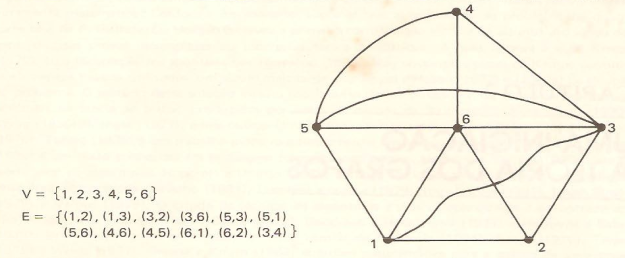
\includegraphics[width=0.7\textwidth]{images/02/fig1.png}
    \end{tabular}
  \end{center}
  \caption{\label{fig:1} Um grafo $G(V,E)$ e sua representação geométrica.}
  \source{Szwarcfiter~\cite{Szwarcfiter1986grafos}.}
\end{figure}


\begin{easylist}
& Vértices: são os elementos de $V$.
& Arestas: são os elementos de $E$.
& Grafo trivial: é um grafo onde $|V| = 1$.
& Vértices adjacentes: dois vértices $v, w$ são ditos adjacentes quando existe uma aresta $e$ tal que $e = (v, w)$; em outras palavras, quando alguma aresta incide em $v$ e $w$.
& Arestas adjacentes: são arestas que possuem uma extremidade em comum, ou seja, que incidem em algum vértice em comum.
& Isomorfismo entre grafos: dois grafos $G_1(V_1, E_1)$ e $G_2(V_2, E_2)$, com $|V_1| = |V_2|$, são ditos isomorfos se e somente se (sse) existe uma função bijetora $f:V_1 \mapsto V_2$ tal que $(v, w) \in E_1$ sse $(f(v), f(w)) \in E_2$ para todo $v, w \in V_1$. Ver Figura~\ref{fig:2}.
\end{easylist}


\begin{figure}[hb]
  \begin{center}
    \begin{tabular}{c}
      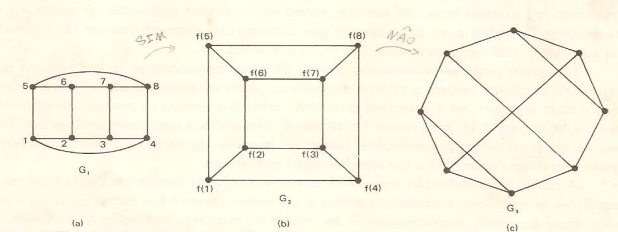
\includegraphics[width=0.8\textwidth]{images/02/fig2.png}
    \end{tabular}
  \end{center}
  \caption{\label{fig:2} Os grafos $G_1$ e $G_2$ são isomorfos um ao outro, mas não a $G_3$.}
  \source{Szwarcfiter~\cite{Szwarcfiter1986grafos}.}
\end{figure}


\begin{easylist}
& Grafo com laços: $G(V,E)$ é um conjunto finito não vazio $V$ e um conjunto $E$ de pares não ordenados de elementos de $V$.
& Grafo dirigido: $G(V,E)$ é um conjunto finito não vazio $V$ e um conjunto $E$ de pares ordenados de elementos de $V$.
& Multigrafo: $G(V,E)$ é um conjunto finito não vazio $V$ e um multiconjunto $E$ de pares não ordenados de elementos de $V$.

& Grau de um vértice $v$ é o número de arestas que incidem em $v$. Laços são contados duas vezes. É denotado por $\operatorname{grau}(v)$.
& Vértice isolado: é um vértice com grau zero.
& Grafo regular de grau $r$: é um grafo em que todos os vértices possuem o mesmo grau $r$.

& Caminho: uma sequência de vértices $v_1, \dots, v_k$ tal que $(v_i, v_{i+1}) \in E, 1\leq i < k$ é denominada caminho de $v_1$ a $v_k$. Seu comprimento é $k-1$.
& Alcance: dizemos que um vértice $v$ alcança um vértice $w$ se existe um caminho de $v$ a $w$.
& Caminho simples: caminho onde todos os vértices de $v_1$ a $v_k$ são diferentes.
& Trajeto: caminho onde todas as arestas são distintas.
& Ciclo: é um caminho $v_1, \dots, v_{k+1}$ em que $v_1 = v_{k+1}$ e $k \geq 3$.
& Ciclo simples: é um ciclo que contém um caminho simples.
& Grafo acíclico: é um grafo que não possui ciclos simples.
& Ciclos idênticos: ciclos obtidos um do outro por uma rotação de seus vértices.
& Caminho Hamiltoniano: caminho que contém cada vértice do grafo exatamente uma vez.
& Ciclo Hamiltoniano: ciclo $v_1, \dots, v_{k+1}$ onde o caminho $v_1, \dots, v_k$ é Hamiltoniano.
& Caminho ou ciclo Euleriano: caminho ou ciclo que contém cada aresta do grafo exatamente uma vez.
  
  
\begin{figure}[!h]
  \begin{subfigure}{.5\textwidth}
    \centering
    \begin{tabular}{c}
      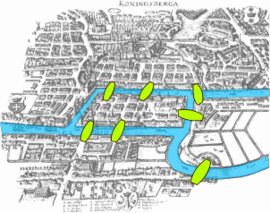
\includegraphics[width=1\textwidth]{images/02/Konigsberg_bridges.png}
    \end{tabular}
    \caption{\label{fig:kon:bridges} Pontes de Konigsberg.}
  \end{subfigure}
  \begin{subfigure}{.5\textwidth}
    \centering
    \begin{tabular}{c}
      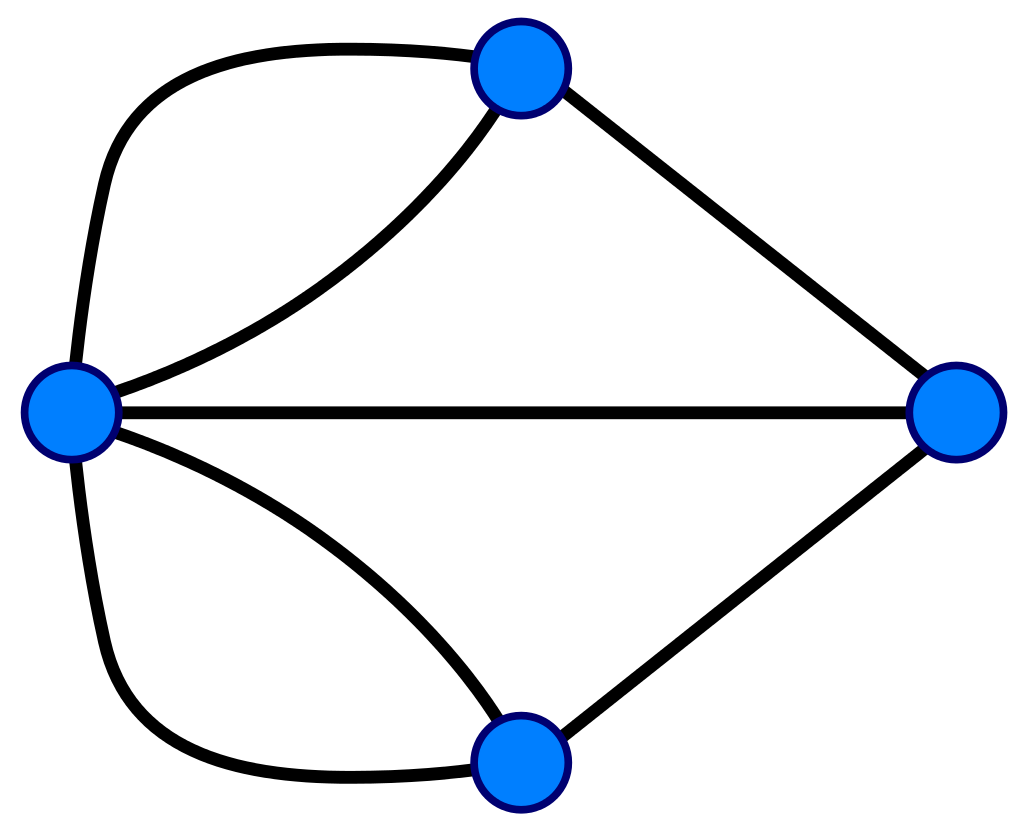
\includegraphics[width=1\textwidth]{images/02/Konigsberg_graph_svg.png}
    \end{tabular}
    \caption{\label{fig:kon:graph} Representação geométrica.}
  \end{subfigure}
  \caption{\label{fig:gray} Existe caminho que percorra todas as pontes uma única vez?}
  \source{Wikipedia.}
\end{figure}






















  

  
\end{easylist}



